% !TEX program = xelatex
% Requires XeLaTeX or LuaLaTeX (fontspec, polyglossia); do not use pdfLaTeX.
\documentclass[11pt, a4paper, twoside]{article}

% =========================================================
% 1. SETUP & PACKAGES
% =========================================================

% --- PDF Handling ---
\usepackage{pdfpages} 
\usepackage{array}
\usepackage{tabularx}
\usepackage{amsmath}
\usepackage{booktabs}
% --- Fonts (XeLaTeX Configuration) ---
\usepackage{fontspec}
\newfontfamily\arial{arial.ttf}

% --- Language ---
\usepackage{polyglossia}
\setmainlanguage{english}
\setotherlanguage{polish}

% --- Margins (Inner 30mm, Outer 20mm) ---
\usepackage{geometry}
\geometry{
    a4paper,
    inner=30mm,
    outer=20mm,
    top=25mm,
    bottom=25mm
}

% --- Spacing (1.15) ---
\usepackage{setspace}
\setstretch{1.15} 
\setlength{\parindent}{0.5cm}
\setlength{\parskip}{0pt}

% --- Page Numbering (Mirrored) ---
\usepackage{fancyhdr}
\pagestyle{fancy}
\fancyhf{}
\fancyfoot[LE,RO]{\thepage} 
\renewcommand{\headrulewidth}{0pt}
\renewcommand{\footrulewidth}{0pt}

% Fix plain pages
\fancypagestyle{plain}{
    \fancyhf{}
    \fancyfoot[LE,RO]{\thepage}
    \renewcommand{\headrulewidth}{0pt}
}

% --- Headings Formatting ---
\usepackage{titlesec}

% Level 1 (Section) - formerly Chapter
% Adjusted to have similar visual weight to your old chapters
\titleformat{\section}
  {\bfseries\fontsize{14}{17}\selectfont} 
  {\thesection}        
  {1em}                      
  {}                         
\titlespacing*{\section}{0pt}{3.5ex plus 1ex minus .2ex}{2.3ex plus .2ex}

% Level 2 (Subsection) - formerly Section
\titleformat{\subsection}
  {\bfseries\fontsize{13}{16}\selectfont}
  {\thesubsection}
  {1em}
  {}

% Level 3 (Subsubsection) - formerly Subsection
\titleformat{\subsubsection}
  {\bfseries\fontsize{12}{15}\selectfont}
  {\thesubsubsection}
  {1em}
  {}

% --- Captions ---
\usepackage{caption}
\DeclareCaptionFont{ninept}{\fontsize{9}{11}\selectfont}
\captionsetup{
    font={ninept}, 
    labelfont=bf, 
    justification=raggedright, 
    singlelinecheck=false,
    skip=5pt
}
\captionsetup[table]{position=top}
\captionsetup[figure]{position=bottom}

% --- Bibliography ---
\usepackage[backend=biber, style=numeric, sorting=nty]{biblatex}
\addbibresource{references.bib}

% --- Links ---
\usepackage{hyperref}
\hypersetup{
    colorlinks=true,
    linkcolor=black,
    citecolor=black,
    urlcolor=black
}

% --- Abstract Environment ---
\newenvironment{abstractspec}{%
    \clearpage
    \thispagestyle{plain}
    \begin{singlespace}
    \fontsize{12}{14}\selectfont
    \noindent
}{%
    \end{singlespace}
    \clearpage
}

% =========================================================
% 2. DOCUMENT CONTENT
% =========================================================

\begin{document}

% --- 1. TITLE PAGE ---
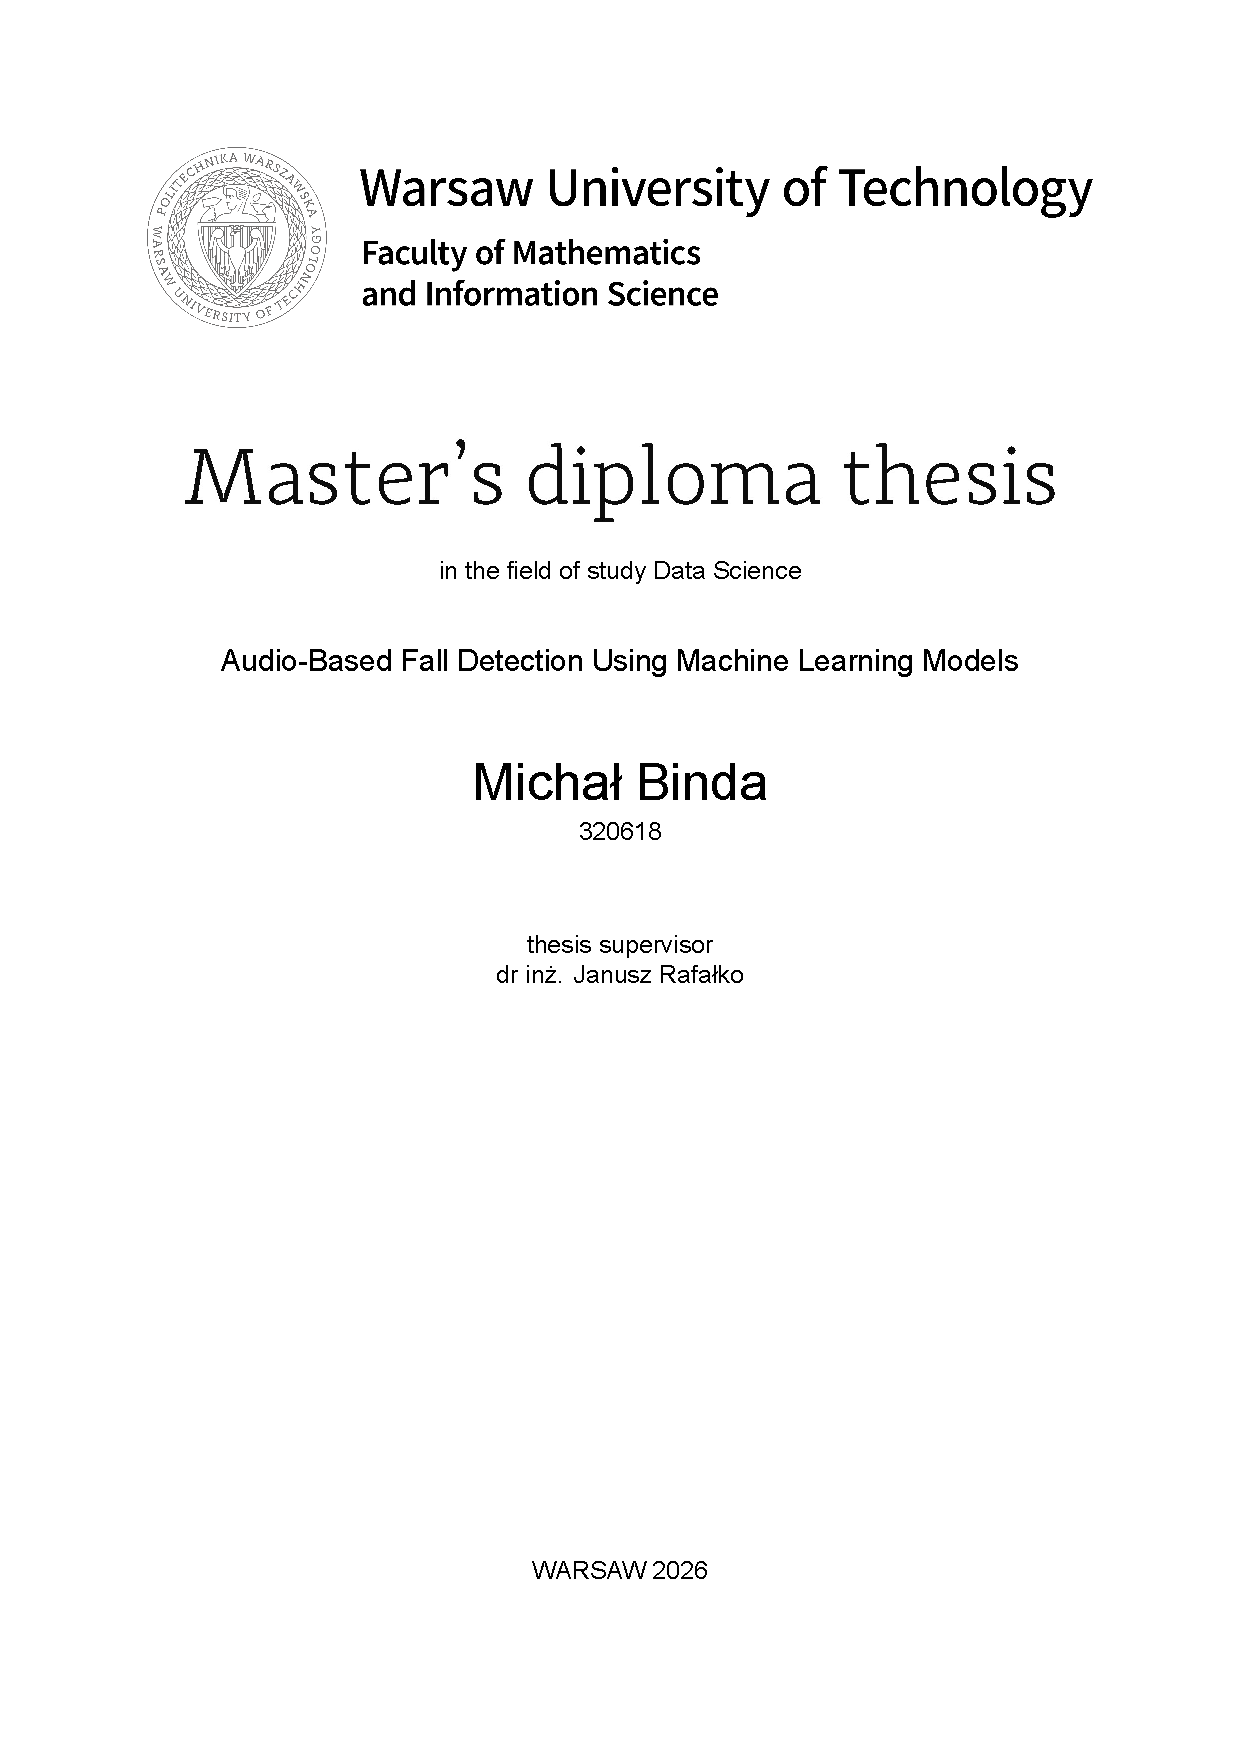
\includepdf[pages=-]{titlepage.pdf}

% --- 2. ABSTRACT (English) ---
\selectlanguage{english}
\setcounter{page}{2} 
\begin{abstractspec}
    \begin{center}
        \textbf{Audio-Based Fall Detection Using Machine Learning Models}
    \end{center}
    \vspace{1em}
    \textbf{Keywords:} machine learning, audio processing, fall detection, classification
    \vspace{1em}
    
    \textbf{Abstract}\\
    %write here
\end{abstractspec}

% --- 3. ABSTRACT (Polish) ---
\selectlanguage{polish}
\begin{abstractspec}
    \begin{center}
        \textbf{Detekcja upadków na podstawie dźwięku przy użyciu modeli uczenia maszynowego}
    \end{center}
    \vspace{1em}
    \textbf{Słowa kluczowe:} uczenie maszynowe, przetwarzanie dźwięku, detekcja upadków, klasyfikacja
    \vspace{1em}
    
    \textbf{Streszczenie}\\
    %write here
\end{abstractspec}

\selectlanguage{english}
\setstretch{1.15}
\normalsize

% --- 4. TABLE OF CONTENTS ---
\tableofcontents
\newpage

% --- 5. MAIN CONTENT (Sections & Subsections) ---

\section{Introduction}

The aim of the thesis is to develop and evaluate methods for fall detection based on sound analysis, with a particular focus on models suitable for deployment on resource-constrained devices.

\subsection{Motivation}
Falls represent a critical health and social problem, particularly in the context of aging societies. They are a major cause of injury, disability, and often death among the elderly. The ability to automatically and rapidly detect a fall is crucial for improving patient prognosis. Unlike solutions based on wearable sensors or video systems, audio-based detection is non-invasive, preserves privacy, and can be implemented using inexpensive, widely available devices, giving the project high practical and commercial potential.
\subsection{Thesis Content Overview}
The work will include:

\begin{itemize}
\item Replication of results from the SAFE (Sound Analysis for Fall Events) article.
\item Construction of lightweight classical and deep models.
\item Implementation of continuous listening and event detection in a two-stage system.
\item Investigation of method robustness to interference.
\item Evaluation of generalization on data from external sources. 
\end{itemize}

The thesis introduces several innovative elements. First, it uses the SAFE dataset, recently published and only publicly available dataset for audio-based fall detection, addressing the lack of open acoustic fall data and enabling reproducibility. Second, the work proposes a custom model architecture optimized for impulsive fall sounds and for deployment on resource-constrained edge devices. Third, it develops a two-stage detection system combining continuous low-power listening with event-triggered classification.


\section{Literature Review}
This chapter provides a comprehensive review of the field of fall detection. Section \ref{intro} describes the clinical context and a brief introduction to different approaches in this field. Section \ref{strate} outlines the main strategies for the development of robust fall detection systems. Firstly, all known strategies are briefly described; then, a detailed analysis of three strategies within the scope of this thesis is presented: wearable-based, vision-based, and, finally, audio-based, which is the main focus of this paper. Thus, the rest of this chapter focuses specifically on this domain. Section \ref{audio} details signal processing techniques used for feeding the data into a classifier. Then, section \ref{machi} presents a comprehensive survey of classifiers used for fall detection, including their features, pros and cons, and results in the research area. Finally, in section \ref{datas}, there is an overview of different types of data gathering techniques and a description of currently available datasets helpful for this thesis.


% The Societal Impact of Falls: Start with WHO statistics. Discuss the aging population (demographics) and the medical consequences of falls (long lie times, hospitalization).
% The Need for Automation: Why manual monitoring fails. The concept of "Golden Hour" in rescue.
% Thesis Relevance: Briefly introduce why current solutions aren't enough, setting the stage for audio analysis.

\subsection{Introduction and Clinical Context}
\label{intro}
Fall detection systems are extremely important nowadays. According to the World Health Organisation, "A fall is defined as an event which results in a person coming to rest inadvertently on the ground or floor or other lower level". They are the second leading cause of unintentional injury deaths worldwide \cite{who2021falls}. Each year, around 37.3 million falls require medical assistance, and 684,000 individuals die from falls. As the population, on average, is getting older, these numbers also grow each year. Adults older than 60 years of age are most prone to these falls, and they are most at Risk. Oftentimes, they require predominantly in-person help. Preventing such events is the best way to neutralize this danger, but in many cases, the fall is impossible to stop. Thus, this paper elaborates on the field of fall detection, with a focus on acoustic sensing. This topic is very broad, and the ideal way to solve fall detection is not straightforward. The task can be divided into 3 subtasks, each of which can be performed in multiple ways: data gathering, data processing, and classification. 

 
\subsection{Fall Detection Strategies}
\label{strate}
Choosing the right strategy is one of the most important factors in building a successful fall detection system. Based on the paper \cite{newaz2023methods} ``The Methods of Fall Detection: A Literature Review'', there are eight main ways to achieve this. A systematic review of over 30,000 articles using resources from Google Scholar, PubMed, and Summon of the Saga University Library has shown that the strategies are as follows: Sound analysis-based, smartphone-based, IoT-based, Wearable device-based, cloud-based, vision-based, Biomedical signal-based, and Kinematic signal-based. Though the research was very broad, this strategic division is not entirely accurate because these strategies often overlap. For instance, Smartphone-based strategies can easily be categorized under Sound analysis, as modern smartphones are universally equipped with microphones. Similarly, a smartphone-based approach can fall under Vision-based strategies when the camera is properly set up. Furthermore, IoT-based strategies overlap with Wearable device-based approaches. An IoT sensor is an electronic device that detects physical changes (such as temperature, motion, light, or humidity), and such a sensor can easily be a wearable device, such as a magnetometer, gyroscope, or accelerometer. Another study \cite{Gattani2026} divides these 8 strategies into 3 categories, as shown in Figure \ref{fig:strategies}: Sensor-Based Methods, Perceptual Sensing Methods, and Communication and Processing Methods. 

\begin{figure}[h!]
    \centering
    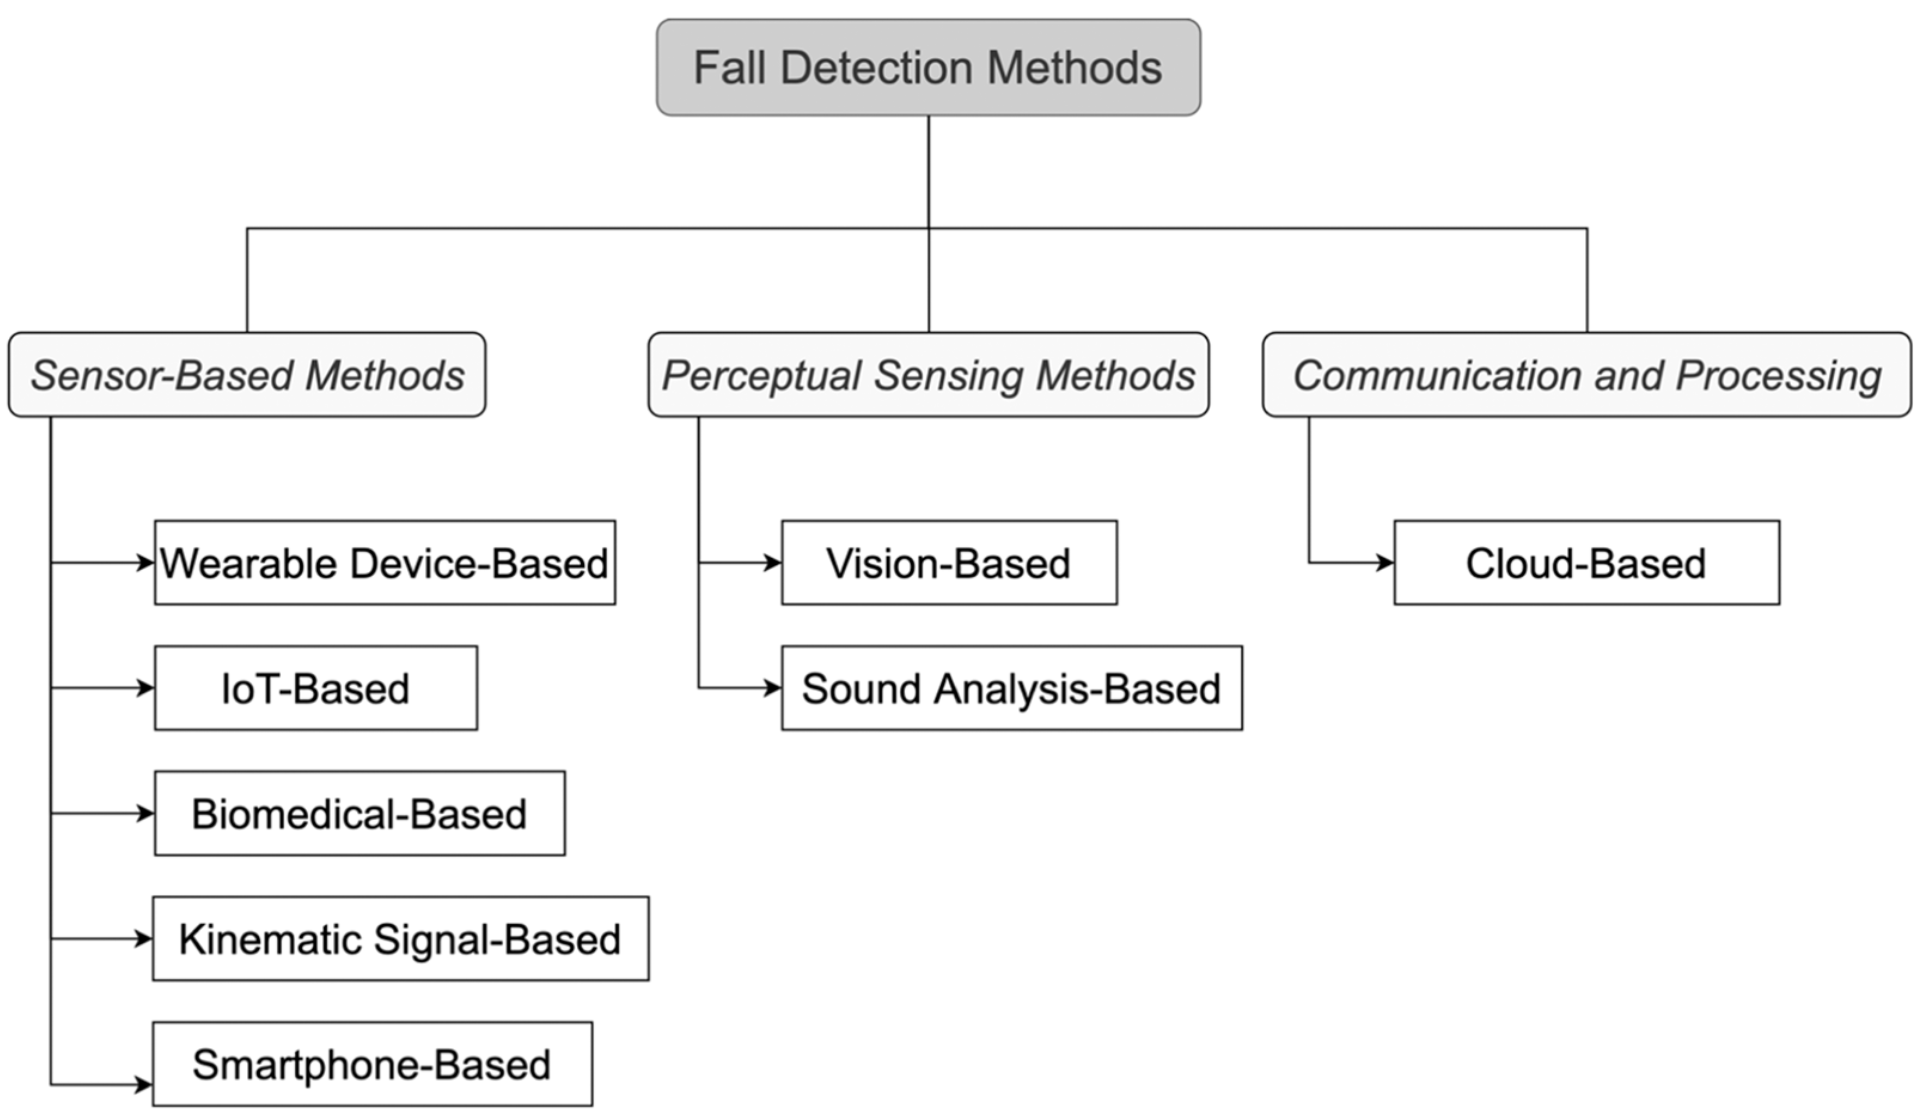
\includegraphics[width=0.9\textwidth]{img/strategies.png} 
    \caption{Taxonomy of fall detection methods categorized into sensor-based, perceptual sensing, and communication and processing approaches \cite{Gattani2026}.}
    \label{fig:strategies}
\end{figure}

For the purposes of this paper, three strategies are outlined, analyzed, and compared:

\begin{itemize}
    \item Wearable Sensors: Accelerometry and Gyroscopy
    \item Vision-Based Systems: RGB Cameras and Depth Sensors
    \item Ambient and Acoustic Sensing: Advantages in Privacy and Compliance
\end{itemize}
The scope of this paper is primarily centered on audio-based fall detection using machine learning models. However, to provide a comprehensive evaluation, we also examine vision-based approaches, which share significant methodological similarities with audio analysis—particularly in the use of Deep Learning architectures. Additionally, we include wearable device-based systems as a representative of sensor-driven strategies, which collectively account for approximately 66\% of the fall detection research landscape. All three methodologies are analyzed and compared in the subsequent sections.

\subsubsection{Wearable Sensors: Accelerometry and Gyroscopy}
The area of fall detection has historically been anchored by wearable sensor technologies, a domain that has improved significantly over the last decade. It has become the baseline for human activity recognition. The fundamental premise of a wearable sensor is its connection to the human body and its ability to measure kinematic forces, specifically proper acceleration and angular velocity, during a fall event. This subsection provides a detailed description of the operational mechanics, algorithmic evolution, and practical limitations of wearable systems, tracing their growth from the simplest heuristics to advanced deep learning methods.
\newline
\newline
The cornerstone of wearable fall detection is the Inertial Measurement Unit (IMU). It typically integrates a triaxial accelerometer and a triaxial gyroscope. The accelerometer measures acceleration along three orthogonal axes. In the context of fall detection, it typically serves as the primary impact detector. The method is based on the free fall period, where the acceleration approaches 0g. The acceleration is measured by the Signal Vector Magnitude, calculated as $\sqrt{A_x^2 + A_y^2 + A_z^2}$, as explained in the paper ``Wearable Fall Detection System with Real-Time Localization and Notification Capabilities. \cite{tseng2025wearable} Reliance solely on acceleration can lead to false positives from other activities, such as jumping. The gyroscope measures rotation rate and is crucial for reconstructing the subject's orientation, which changes rapidly during a fall. By integrating angular velocity over time, algorithms can distinguish between lying down on a bed and an uncontrolled fall, reducing the number of false positives. Research has shown that incorporating gyroscopic data can significantly enhance detection accuracy. Anatomical placement is one of the key decisions for successful fall detection. The waist or lower back (Sacrum) is known to be the optimal location as it is closest to the center of mass. Sensors positioned at this location achieved the highest accuracy (98.42\%), followed by the thigh, ankle, head, chest, and wrist in that order. Another study, ``An Analysis of the Accuracy of Wearable Sensors for Classifying the Causes of Falls in Humans'' \cite{aziz2011analysis}, examined differences between single- and multi-sensor configurations. For example, a three-node accelerometer array (placed on the left ankle, right ankle, and sternum) achieved 96\% sensitivity and 98\% specificity in distinguishing the causes of falls, whereas the single waist marker provided only 54\% sensitivity. Nevertheless, consumer preference has driven the market towards wrist-worn devices. While very comfortable to wear, the wrist is a challenging location for fall detection because arm movements are highly variable and often unrelated to the trunk's orientation. Gesturing or clapping can generate acceleration spikes that mimic a fall impact. To mitigate this, modern algorithms employ filtering techniques to decouple arm motion from body motion. Similarly, head-worn sensors integrated into smart glasses have been explored, using complementary filters to eliminate angle measurement instability and drift, as stated in the paper \cite{tseng2025wearable}. The processing of wearable sensor data has undergone an evolutionary trajectory, moving from threshold-based to automated feature learning. 
\newline
\newline
\textit{Threshold-Based Algorithms:} A typical logic flow might trigger a fall alarm if a certain feature (e.g. acceleration) exceeds a certain value (e.g. 2.5g). These methods are computationally efficient, making them ideal for low-power microcontrollers with limited battery life. For example, in \cite{tseng2025wearable}, a low-complexity algorithm based on a finite-state machine was successfully deployed on an NB-IoT device, achieving 97.9\% sensitivity in outdoor environments while filtering out activities like running and stair climbing. However, the reliance on fixed thresholds makes these algorithms prone to false false positives in a new environment. To overcome these limitation, researchers began implementing algorithms based on supervised machine learning. This approach involves extracting statistical features (e.g. mean and variance) from sliding windows of data. This data was later fed to classifiers. Support Vector Machines are highly effective in high-dimensional spaces. Decision Trees and Random Forests are known for interpretability and robustness against overfitting. Naive Bayes classifiers, which are easy to implement and computationally efficient, perform well even with less training data. In the research ``Fall Detection and Monitoring using Machine Learning: A Comparative Study'' \cite{edeib2023comparative}, these models achieved accuracies of 95\%, 97\%, and 91\%, respectively. The current state of the art leverages Deep Learning to automate feature engineering. Instead of manually selecting statistical features, deep learning models learn hierarchical representations directly from the raw data. These models have been widely applied to classification tasks and have achieved superior results. In the paper ``An Effective Deep Learning Framework for Fall Detection: Model Development and Study Design'' \cite{zhang2024effective}, the best outlined methods were: Convolutional Neural Networks (CNN), Recurrent Neural Networks such as Long Short-Term Memory (LSTM), and Dual-Stream Convolutional Neural Network Self-Attention. Convolutional Neural Networks, originally designed for image processing, have been adapted for time-series data (1D-CNNs) or by treating sensor spectrograms as images (2D-CNNs). These models have been widely applied in classification tasks for human activity recognition.
\newline
\newline
Despite major improvements over the last decade, wearable devices have their challenges and limitations. Research indicates a significant drop in utility when moving from controlled studies to real-world applications. Elderly individuals often forget to wear the sensors or remove them during high-risk activities, such as cooking or bathing. There is always a need to charge these sensors, and the burden of maintenance remains a barrier for users with dementia or cognitive decline. In summary, despite the evolution of wearable sensors into highly sophisticated ML-driven systems, these approaches are marked as fragile due to their high dependence on user compliance.

\subsubsection{Vision-Based Systems: RGB Cameras and Depth Sensors}
Vision-based systems are a rapidly growing area of fall detection systems. They are contactless and passive.  Wearable sensors' limitations, such as charging or remembering to wear the device, are eliminated. When successfully set up, these systems provide continuous monitoring without active user participation, capturing motion, posture, and environmental context. This subsection explores the two primary categories of vision sensing: standard RGB imagery and depth-sensing technologies, describing their methodology, results, and limitations.
\newline
\newline
Single RGB cameras capture 2D color image sequences and have been studied by many researchers. The classifiers rely on the ratio of width to height, as well as other features such as motion and the moving object's centroid. Although they are easy to set up and inexpensive, they are known to be fragile and prone to confusion. They do not view the whole environment and can be easily blocked by objects. Thus, this method is often treated as a baseline. To overcome the problem of occlusion (objects covering part of an image), 3D-based methods were introduced. Such methods include:

\begin{itemize}
    \item Multiple RGB Cameras
    \item Depth Cameras
\end{itemize}

The first approach requires multiple cameras, which makes the setup significantly more expensive and complex. This method also presents privacy limitations. Recording elderly people can create discomfort and a sense of lost dignity. To overcome this issue, researchers have turned to RGB-D sensors. They differentiate red, green, and blue colors and depth, where each pixel represents a distance value rather than just color intensity. The privacy aspect is well described in the paper ``Privacy preserving automatic fall detection for elderly using RGBD cameras'' \cite{zhang2019privacy}, which clearly states that this method preserves privacy. The cameras can also track human skeletal joints. Although this method was initially the most expensive, these sensors are now more available and affordable. Based on the paper ``A survey on vision-based fall detection'' \cite{zhang2006survey}, all three methods can be useful, and none is inherently superior to the others in detecting falls.
\newline
\newline
Early vision-based methods relied on background subtraction and bounding-box analysis. A fall could be detected if the bounding box's shape exceeded a threshold. This approach had multiple limitations. Computer vision was subsequently revolutionized by machine learning and deep learning methods. Various studies proved these methods to be reliable and robust, given the right amount of quality data. The most popular method in computer vision is the Convolutional Neural Network (CNN), which is designed for image processing. The paper ``A vision-based approach for fall detection using multiple cameras and convolutional neural networks: A case study using the UP-Fall detection dataset'' \cite{espinosa2019vision} examined the effectiveness of a proposed CNN architecture against baseline methods such as Support Vector Machine, Random Forest, and Multi-Layer Perceptron. The best configuration was the CNN network, proving the superiority of Deep Learning algorithms. An ensemble of this network proved to have even better results, reaching an accuracy of 100\%, as shown in the paper ``Deep Learning for Fall Detection: Three-Dimensional CNN Combined With LSTM on Video Kinematic Data'' \cite{lu2018deep}.
\newline
\newline
Although vision-based methods address the limitations of wearable sensors, such as the maintenance burden on the user, they come at the cost of privacy concerns and higher costs. While a single RGB camera is easy to use, it is limited by environmental factors. More advanced approaches, like Multiple RGB Cameras or RGB-D Cameras, yield better results but are significantly more expensive and complex. The current state of research clearly shows that deep learning models are the optimal configuration, with many researchers arguing that CNNs are the best model.


\subsubsection{Ambient and Acoustic Sensing: Advantages in Privacy and Compliance}

While wearable approaches struggle with user compliance, and vision systems cross privacy boundaries, ambient and acoustic sensing overcome all these issues. The strategy focuses on extracting information from sound waves and vibrations to understand context, events, or human activity, often without requiring direct user interaction. Interest in this field has grown significantly in fall detection. Acoustic sensing represents a highly promising frontier that excels in broad coverage, low cost, and privacy preservation. This subsection details the physics behind the acoustic signature of a human fall and the advanced methods used for preprocessing and classification.

During a typical fall, a human rapidly impacts another object. This event is characterized by the production of a transient signal of high energy, especially when the patient hits a wooden floor or parquet in an indoor environment. Usually, it is followed by a period of silence, during which the person who fell is confused and processes the cause-and-effect of the fall. The acoustic detection of such an occurrence can be done in two ways:

\begin{itemize}
    \item \textbf{Impact Transient:} The impact of a body hitting the floor generates a sound wave with a sudden onset and high amplitude. Unlike continuous sounds like speech or music, a fall is an impulse event with significant energy distributed across low frequencies. Research has shown that analyzing these shockwaves can be very effective in detecting falls. The goal is to classify their temporal and spectral patterns using pattern recognition algorithms. In the paper ``Fall detection of the elderly through floor vibrations and sound'' \cite{litvak2008fall}, it has been proven that such an approach can be further improved with floor vibration sensing. Using pattern recognition algorithms, they achieved 95\% sensitivity and 95\% specificity for human fall detection.
    \item \textbf{Ultrasonic Doppler Sensing:} This approach requires the system to actively flood a room with high-frequency sound waves and analyze how those waves bounce back in order to capture the Doppler shift caused by the fall. Consequently, the algorithm can measure velocity and distinguish between the user sitting down and falling. The microphone records the reflected signal, and by using machine learning or deep learning techniques, it classifies the current human condition. Such an approach has been described in the paper ``Fall Detection via Inaudible Acoustic Sensing'' \cite{lian2021fall}, where the authors used Singular Value Decomposition to reduce the feature dimension and a Hidden Markov Model to train and classify the data. In an indoor environment, young participants achieved an F1-score of up to 98\%.
\end{itemize}

The key process of the acoustic-based strategy is data retrieval. The results heavily depend on the correct extraction of robust features that can discriminate the specific fall sound. This can be done using:

\begin{itemize}
    \item \textbf{Mel-Frequency Cepstral Coefficients:} These are essential features in audio processing, representing the short-term power spectrum of a sound by modeling human hearing's non-linear frequency perception.
    \item \textbf{Gammatone Cepstral Coefficients:} These are advanced audio features, inspired by human hearing, that use Gammatone filters instead of Mel filters to analyze audio. They better capture spectral envelopes, especially at low frequencies, leading to higher performance in tasks such as speaker verification, fall detection, and non-speech audio classification by modeling auditory perception more closely.
    \item \textbf{Spectrograms:} A visual representation of the spectrum of frequencies in a signal as it changes over time. It is a two-dimensional graph with time on the horizontal axis, frequency on the vertical axis, and amplitude represented by color or intensity. They allow the model to learn complex patterns, such as the specific spectral decay of a fall.
\end{itemize}

These methods are elaborated in Section~\ref{sec:signal}.
\newline
The last step to create a complete process for acoustic event detection is to choose a classifier. The signal feature space typically requires an advanced classifier capable of distinguishing subtle changes and complex patterns. Thus, machine learning techniques are heavily used in this area. Both classical Machine Learning Models, such as Support Vector Machines, k-Nearest Neighbors, and Decision Trees, and more complex Deep Learning Models (e.g., CNN, LSTM, Transformers) are being widely used and tested. A comprehensive survey is available in section \ref{mlm}. 
\newline
\newline

Though this branch has promising results, it also has its own limitations. The major ones are: 
\begin{itemize}
    \item \textbf{Source Localization in Reverberant Environments:} In highly reflective environments such as a bathroom or a small kitchen, the sound wave reflects from surfaces like the floor or furniture, and the same signal is often received over more than one path. This effect, known as multipath propagation, twists the Time Difference of Arrival, reducing the sharpness of the onset detection.
    \item \textbf{Non-Line-of-Sight Attenuation:} In some environments, the sound waves are gathered from multiple rooms. This may result in the attenuation of high-frequency components when they pass through walls or obstacles. Thus, it is advisable to put a 
    \item \textbf{Event Overlap:} The sound wave is gathering information from the whole environment, making it hard to be noise-free. Sounds like television, chatter, or cooking can distort the spectral components, making it harder for the model to make the correct prediction.
    \item \textbf{Data Availability:} Currently, there aren't many available datasets for audio-based human falls. This limits model robustness and makes it much harder to generalize. There are methods to overcome this issue, described in section \ref{datas}.
\end{itemize}

In summary, acoustic-based algorithms for fall detection are a very promising method and could help revolutionize the current state of the research area. They overcome the limitations of computer vision and wearable sensors. They are a low-cost system that can be configured in any apartment or house. With a limited number of microphones, the system can cover an entire room or even monitor adjacent spaces. This technique is also user-friendly and is entirely passive. It does not require any maintenance, such as charging the battery or pressing buttons. Finally, it allows the user to feel comfortable, unlike a camera, which captures intimate visual details. In practice, the methodology has shifted from Hidden Markov Models to advanced Deep Learning architectures, making the field's current state still a developing area. The limitation of this domain is mainly the source localization, multipath propagation, attenuation, event overlap, and scarcity of the data. 

%todo - write about cons Noise interference, lack of data



\subsubsection{Comparative Analysis of Detection Modalities}
To understand the current state of Audio-based Fall Detection, it is necessary to compare it with the other main modalities. This section outlines the advantages and disadvantages of each modality.

\textbf{Wearable Systems:}
\begin{itemize}
    \item \textbf{Advantages:} Wearables are unaffected by lack of lighting or line-of-sight occlusion and can achieve the highest theoretical accuracy due to their direct measurement of body motion. They are robust and an extensively examined practice.
    \item \textbf{Disadvantages:} They require high user compliance. The maintenance burden relies heavily on the patient, often an elderly individual who may forget their duties. When the device is not worn, it yields 0\% accuracy.
\end{itemize}

\textbf{Vision Systems:}
\begin{itemize}
    \item \textbf{Advantages:} They are the best method to extract contextual data. They provide an explanation of a fall, which might help to reduce such events in the future. They are most effective at distinguishing soft falls from sitting or lying down, where small gestures, such as uncontrolled hand movements, are the only way to detect a fall.
    \item \textbf{Disadvantages:} Cameras are a more expensive implementation than wearable or audio sensors. Furthermore, a single camera might not be enough to cover every corner. To ensure the environment is well monitored, the system needs multiple devices, which further increases the cost. The accuracy degrades with poor lighting and does not work well at night. Moreover, the biggest issue is user privacy. Elderly people are not easily persuaded to have a camera installed in intimate rooms like bedrooms or bathrooms, which are the most common places for falls.
\end{itemize}

\textbf{Acoustic Systems:}
\begin{itemize}
    \item \textbf{Advantages:} Acoustic systems bridge the gap. They are contactless, passive, and privacy-preserving. They do not require user maintenance and reduce the cost of setup. They can be easily installed in every room without the user fearing any disturbance.
    \item \textbf{Disadvantages:} They are susceptible to environmental noise pollution such as music, radio, or television. They lack precise, clean data, which is readily available from wearable sensors. The lack of data must be overcome by establishing an advanced, well-architected model.
\end{itemize}

\begin{table}[htbp]
\centering
\caption{Comparison of Fall Detection Technologies}
\label{tab:fall-detection}
\renewcommand{\arraystretch}{1.5} % Increases row height for readability
\begin{tabular}{|p{2.5cm}|p{3.5cm}|p{3.5cm}|p{3.5cm}|}
\hline
\textbf{Feature} & \textbf{Wearable Sensors (IMU)} & \textbf{Vision-Based (RGB/Depth)} & \textbf{Acoustic/Ambient Sensing} \\ \hline
Primary Data Source & Acceleration, Angular Velocity & Image Sequences, Depth Maps & Sound Waves, Vibrations, Ultrasonic Reflections \\ \hline
Intrusiveness & High (must be worn/charged) & High (perceived surveillance) & Low (perceived as passive) \\ \hline
Privacy Risk & Low (data is abstract) & High (potential for visual identification) & Low to Medium (risk of speech recording) \\ \hline
Key Limitation & User Compliance (forgetting to wear) & Occlusion \& Privacy & Background Noise \& Localization \\ \hline
Blind Spots & None (moves with user) & Furniture, Walls, Low Light & High Noise Environments \\ \hline
Cost & Low (device cost) & Medium to High (cameras + GPU) & Low (microphones are ubiquitous) \\ \hline
Detection Basis & Impact \& Orientation Change & Pose Change \& Velocity & Impact Sound \& Distress Speech \\ \hline
Suitable for Bathroom & Yes (if waterproof/worn) & No (privacy/humidity issues) & Yes (highly effective, non-intrusive) \\ \hline
\end{tabular}
\end{table}

The table \ref{tab:fall-detection} provides a comparative analysis of Fall Detection Modalities. The literature and observations suggest that multimodal fusion might be the answer to the problems of all three approaches, where the strengths of one system compensate for the weaknesses of another. Combining video pose estimation with audio event detection has been shown to significantly reduce false positives.

Nowadays, Audio-Visual fusion is the most promising strategy for Fall Detection, and many researchers focus heavily on this approach. The two modalities together cover around 41.5\% of the fall detection strategies in research papers found in Google Scholar from 1990 to 2022 \cite{newaz2023methods}. A recent paper published in October 2025, ``Audio-visual multimodal fall detection to ensure the safety of elderly people in intelligent buildings: an innovative approach using LSTM, CNN, and a shallow neural network,'' tested both components separately and compared them with a fusion strategy. Despite the single components achieving good results—the Audio component reaching 93.88\% accuracy and the Vision-based component reaching 96.95\%—fusing audio and visual modalities achieved 99.90\%, which is far superior. Though this method has remarkable results, it also faces challenges. These are mainly related to cost-complexity issues, which are well described in the paper ``Performance, challenges, and limitations in multimodal fall detection systems: A review'' \cite{9459770}.
\newline

In conclusion, while wearable sensors are currently the most common approach for Human Fall Detection, and vision systems offer the best contextual understanding, acoustic sensing represents a promising, growing field. Although it has its challenges, it provides a solution that addresses the privacy issue and does not require user maintenance. This thesis focuses on exploiting this modality to create a robust, privacy-centric fall detection system. The following three chapters elaborate on this approach in detail. First, the fundamentals of audio signal processing for event detection are introduced, with an emphasis on feature extraction and impact transient analysis. Next, machine learning models for audio-based classification are presented and discussed. Finally, the datasets used in this work and the evaluation metrics employed to assess system performance are described.

\subsection{Audio Signal Processing for Event Detection}
\label{audio}
This section provides a survey of Audio Signal Processing, which was previously introduced. The goal of this section is to provide an overview of current research on audio processing, with a focus on techniques and mechanics relevant to a fall event, including normalization, resampling, noise reduction, and feature extraction.

\subsubsection{Signal Characteristics of a Fall}
\label{sec:signal}
To design an audio-based algorithm for fall detection, one must first understand the physics of the impact and its acoustic properties. The mechanics of impact are more complex than initially anticipated. A fall is an impulsive, transient event. Even though it is a sudden movement involving a physical strike on the floor, research shows it possesses unique characteristics. It is characterized by a non-periodic burst of energy that lasts 100 to 500 milliseconds. The duration of the fall sound is often elongated by multiple joints hitting the floor with small delays. These unique features help differentiate a human fall from the impact of a rigid object, such as a ceramic mug or a metal spoon, which produces a singular, high-frequency spike.

Acoustic analysis reveals that the majority of the power in a fall signal is concentrated in the low-frequency bands, typically below 500 Hz. According to the paper ``Time-Frequency Analysis of Daily Activities for Fall Detection’’ \cite{huynh2021time}, a fall’s structural resonances are often in the range of 20 Hz to 100 Hz. High frequencies are damped by the soft tissue of the body, such as fat or skin. Consequently, from a theoretical standpoint, a fall can be distinguished by the dominant frequency range and the decay profile, as shown in Table \ref{tab:acoustic_events}.

In reality, the signal is accompanied by background noise, which makes prediction significantly harder. Although stationary noise, such as that produced by household appliances (e.g., HVAC, refrigerators), which manifests as constant horizontal bands, is easily eliminated during preprocessing, transient interference is much more challenging for classifiers. For an algorithm to differentiate sounds such as door slams, heavy footsteps, or clapping hands from a fall, a well-architected preprocessing pipeline is necessary.

\begin{table}[htbp]
\centering
\small % Reduces font size slightly to fit content better
\caption{Characteristics of Common Acoustic Events}
\label{tab:acoustic_events}
\renewcommand{\arraystretch}{1.5} % Adds vertical padding for readability
% Set table width to \textwidth. 
% 'l' is for the first column (keeps it compact).
% 'X' is for the other columns (allows them to wrap text automatically).
\begin{tabularx}{\textwidth}{|l|X|X|X|}
\hline
\textbf{Acoustic Event} & \textbf{Temporal Characteristic} & \textbf{Dominant Frequency} & \textbf{Decay Profile} \\ 
\hline
Human Fall 
& Impulsive, Multi-stage 
& Low (20 Hz -- 500 Hz) 
& Slow, Damped ($>300$ ms) \\ 
\hline
Dropped Object 
& Impulsive, Single-stage 
& High ($>1$ kHz) 
& Fast ($<100$ ms) or Ringing \\ 
\hline
Door Slam 
& Impulsive 
& Mid-Low (100 Hz -- 1 kHz) 
& Moderate \\ 
\hline
Speech 
& Intermittent, Periodic 
& Mid (300 Hz -- 3.4 kHz) 
& Variable \\ 
\hline
\end{tabularx}
\end{table}

\subsubsection{Preprocessing Techniques}
Audio data preprocessing is a key technique in machine learning methodologies. Multiple techniques are used to clean and prepare the data for further analysis. This section details noise reduction, resampling, and normalization—the key processes for a successful preprocessing pipeline.

Filtering background noise ensures the model focuses on the relevant signal. A classical approach to denoising is \textbf{Spectral Subtraction}. It is widely used and assumes that noise is additive and stationary. It estimates the noise spectrum and subtracts it directly from the noisy signal spectrum \cite{pranami2016audio}:

\begin{equation}
\left| \hat{S}(\omega) \right| = \left| Y(\omega) \right| - \left| N(\omega) \right|
\end{equation}

where:
\begin{itemize}
\item $Y(\omega)$ is the noisy signal spectrum
\item $N(\omega)$ is the estimated noise spectrum
\item $\hat{S}(\omega)$ is the enhanced (noise-reduced) signal spectrum
\end{itemize}

It is very effective for removing constant hums, but in rare cases, it can produce musical noise artifacts. Another strategy for \textbf{Noise Reduction} is \textbf{Wiener Filtering}. It uses statistical estimation to adapt filter parameters dynamically for minimum mean square error between clean and noisy signals \cite{pranami2016audio}:

\begin{equation}
\hat{S}(\omega) = H(\omega),Y(\omega)
\end{equation}

with the Wiener filter defined as:

\begin{equation}
H(\omega) = \frac{P_S(\omega)}{P_S(\omega) + P_N(\omega)}
\end{equation}

where:
\begin{itemize}
\item $Y(\omega)$ is the noisy signal spectrum
\item $P_S(\omega)$ is the power spectral density of the clean signal
\item $P_N(\omega)$ is the power spectral density of the noise
\item $\hat{S}(\omega)$ is the enhanced signal spectrum
\end{itemize}

Even though spectral subtraction is easy to implement and effective, Wiener filtering is often optimal and yields better performance on non-stationary noise. Therefore, it is often preferred for fall detection, where noise typically originates from sources such as traffic or television.

\textbf{Resampling} converts samples from their original rate to the target rate. Standardizing the sampling rate ensures consistency and maintains the same shape of time–frequency representations. Higher sampling rates increase memory usage and processing time. Downsampling to a lower rate reduces the number of samples per second, thereby lowering the computational cost.

\textbf{Normalization} scales the amplitude of the audio signal. It ensures that the model is not biased towards signals at closer ranges, which typically exhibit higher energy levels. Popular normalization techniques include Min–Max and Z-score normalization.

\textbf{Min-Max Normalization} scales the waveform amplitude to a fixed range, typically $[-1, 1]$. Dividing by the maximum absolute amplitude removes absolute loudness information, making the data adaptable to recording distance.

\begin{equation}
x_{\text{norm}}[n] = \frac{x[n]}{\left| \max(x) \right|}
\end{equation}

where:
\begin{itemize}
\item $x[n]$ is the original discrete-time audio signal,
\item $x_{\text{norm}}[n]$ is the normalized signal,
\item $\max(x)$ denotes the maximum absolute amplitude of the signal.
\end{itemize}

Another normalization technique is \textbf{Z-Score Standardization}, in which the mean value of the signal is subtracted from each sample, and the result is scaled by the standard deviation:

\begin{equation}
x_{\text{std}}[n] = \frac{x[n] - \mu}{\sigma}
\end{equation}

where:
\begin{itemize}
\item $x[n]$ is the original discrete-time audio signal,
\item $x_{\text{std}}[n]$ is the standardized signal,
\item $\mu$ is the mean value of the signal samples,
\item $\sigma$ is the standard deviation of the signal samples.
\end{itemize}

This method is robust against outliers, preventing features with larger magnitudes from dominating the learning process.

\subsubsection{Feature Extraction: Time-Domain Features}
The key procedure for complex analysis in Audio Processing is Feature Extraction. This section outlines the two main methods used for feature extraction in the time domain: Zero-Crossing Rate and Short-Time Energy.

\textbf{The Zero-Crossing Rate (ZCR)} is defined as the rate at which the signal changes sign during a frame. It is the number of times a signal changes from positive to negative or vice versa and is defined by the equation \cite{babaee2017overview}:

\begin{equation}
ZC = \frac{\sum_{n=1}^{N} \left| \mathrm{sgn}[x(n)] - \mathrm{sgn}[x(n-1)] \right|}{2N}
\label{eq:zcr}
\end{equation}

where $\mathrm{sgn}[x(n)]$ is the sign function, defined as:

\begin{equation}
\mathrm{sgn}[x(n)] =
\begin{cases}
1, & \text{if } x(n) \ge 0 \\
-1, & \text{if } x(n) < 0
\end{cases}
\label{eq:sign_function}
\end{equation}

A high-frequency signal will change sign frequently, whereas a low-frequency signal will do so rarely. Consequently, the method is excellent for distinguishing falls from high-frequency events like glass breaking or dropping cutlery.

Another technique used for feature extraction is \textbf{Short-Time Energy (STE)}. While ZCR measures frequency characteristics, STE measures signal amplitude within the frame, commonly known as ``loudness.‘’ It is primarily used to distinguish silence from speech. It is defined by the equation \cite{rabiner1978digital}:

\begin{equation}
E_n = \sum_{m} [x[m] \cdot w[n-m]]^2
\end{equation}

where:
\begin{itemize}
\item $x[m]$ is the signal sample at time index $m$,
\item $w[n-m]$ is the window function (e.g., Hamming or Hann) centered at frame index $n$,
\item $E_n$ is the short-time energy of the signal at frame $n$.
\end{itemize}

In the context of fall detection, STE can be very useful for detecting a period containing an event and can serve as a trigger to activate more complex classifiers. Research has shown that both Zero-Crossing Rate and Short-Time Energy can improve fall detection classifiers. ZCR can distinguish low and high-frequency signals, whereas STE is useful as a trigger tool.

\subsubsection{Feature Extraction: Frequency-Domain Features}
Although Time-Domain features are extremely helpful for human activity recognition, they can be prone to false positives because they lack advanced spectral information. Consequently, frequency-domain features are an excellent choice to eliminate such cases. They are derived from the Discrete Fourier Transform (DFT) or Fast Fourier Transform (FFT) of the signal frames. They describe the composition of the sound, providing features such as Spectral Centroid and Spectral Bandwidth, which are described in this subsection.

\textbf{Spectral Centroid} calculates the average point of the spectral energy. It represents the dominant signal frequency over time and is formulated as follows \cite{Babaee2017}:

\begin{equation}
SC = \frac{\int_{0}^{\bar{\omega}} \omega |F(\omega)|^{2} d\omega}{E}
\end{equation}

where:
\begin{itemize}
\item $SC$: The Spectral Centroid, representing the center of audio frequency distribution.
\item $\omega$: The frequency (or center frequency $\omega_k$).
\item $E$: The energy of the audio signal.
\item $|F(\omega)|^{2}$: The power spectrum of the audio signal.
\item $\bar{\omega}$: The upper limit of the frequency range.
\end{itemize}

Because of the mechanics of a human fall, the spectral centroid is a robust technique for distinguishing falls from dropping small objects such as keys. A human fall is characterized by low frequencies (below 500 Hz); therefore, it has a distinctively low spectral centroid. Even if a key drop event has the same duration and energy as a fall—which might confuse STE and ZCR features—the key drop will have a significantly higher spectral centroid.

Another frequency-based feature is \textbf{Spectral Bandwidth}. It measures the width of the spectrum relative to the signal centroid. A fall typically has a wider bandwidth, whereas an event such as a phone ring has a very narrow bandwidth. This feature helps filter out electronic alerts that might trigger energy-based methods.

\subsubsection{Deep Dive: Time-Frequency Representations}
While statistical features like ZCR and Spectral Centroid are effective for lightweight classifiers such as Decision Trees or SVMs, they inevitably compress the data, impeding the classifiers from utilizing more complex architectures. Spectral characteristics or Mel-frequency Cepstral Coefficients (MFCCs) can provide a much more comprehensive and sophisticated analysis, making them suitable for complex methodologies. Therefore, this section describes in detail the logic, performance metrics, and observations behind them.

A \textbf{Mel Spectrogram} \cite{kaur2022fall} is a visual representation of the frequency spectrum of a sound signal. It is calculated by applying a Short-Time Fourier Transform (STFT) to the signal, converting it from the time domain to the frequency domain. The resulting spectrogram is then mapped to the Mel scale, a perceptual scale of pitches judged by listeners to be equally spaced. The Mel scale is uniquely advantageous for fall detection, as it focuses on low frequencies and allocates more bins to the region where the fall signal occurs. Finally, to match the human perception of loudness, a logarithmic operation is applied. The key parameters for the quality and resolution of a Mel spectrogram are:

\begin{itemize}
\item \textbf{Window Type}: A function applied to each frame to reduce spectral leakage, typically a Hann window.
\item \textbf{Mel Bins (M)}: The number of frequency bands used. It determines the dimensionality of the feature vector and the frequency axis.
\item \textbf{Hop Length}: The number of samples between frames. Shorter hop lengths improve temporal resolution but increase computational cost.
\end{itemize}

A \textbf{Mel-Frequency Cepstral Coefficient (MFCC)} \cite{babaee2017overview} is the most popular feature extraction method in speech recognition. It provides a compact representation of the spectral envelope. To calculate it, one follows the same steps as for Mel spectrograms and then applies the Discrete Cosine Transform (DCT) to the log-Mel energies. This transformation decorrelates the features, making them invaluable for Deep Learning methods such as CNNs.

Whereas MFCCs are ideal inputs for lightweight statistical classifiers, Mel Spectrograms are preferred for deep learning architectures. Research in audio-based fall detection shows that, when computational resources allow, Convolutional Neural Networks (CNNs) are the preferred technique, prioritizing Mel spectrograms over other feature extraction methods. For instance, recent work by Al-Shammari et al. \cite{alshammari2025} demonstrated that using Mel spectrograms in a CNN backbone can achieve over 93\% accuracy in detecting falls, outperforming traditional 1D feature analysis. Thus, MFCCs remain the standard for resource-constrained environments, as shown in \cite{guillem2013improving}, where low latency and minimal memory usage are critical.

\subsection{Machine Learning Model Overview}
\label{machi}
\label{mlm}
Once acoustic features have been 
extracted from the raw audio waveform, whether they are simple time-domain statistics like ZCR or complex spectral representations like Mel-spectrograms, the next critical phase is classification. This is the key process for detecting fall events, for which one can use various machine learning models. The decision of which model to use is not merely a matter of maximizing accuracy but also involves considering limitations, such as a lack of generalization or high time and cost complexity. These systems must operate in real time, maximizing accuracy while minimizing false alarm rates, which are a burden on caregivers.

As summarized in Table \ref{tab:audio_features}, there is a direct correlation between the complexity of the feature representation and the recommended machine learning architecture. While statistical methods (ZCR, STE, MFCCs) are suitable for lightweight Decision Trees, k-NN, and SVMs, high-dimensional Mel-spectrograms require the hierarchical learning capabilities of Deep Neural Networks. This section analyzes this technological spectrum, evaluating the models across various datasets and outlining their limitations.

\begin{table}[h!]
\centering
\small % Reduces font size to fit content
\renewcommand{\arraystretch}{1.5} % Increases row height for readability
\caption{Comparison of Audio Feature Representations and Model Architectures}
\label{tab:audio_features}
% tabularx set to \textwidth to match page margins
% 'X' columns expand to fill space and wrap text automatically
\begin{tabularx}{\textwidth}{|p{2.2cm}|p{2.5cm}|p{2.2cm}|X|X|}
\hline
\textbf{Feature Rep.} & \textbf{Info. Content} & \textbf{Dims} & \textbf{Rec. Architecture} & \textbf{Rationale} \\ 
\hline
\textbf{ZCR / STE / Centroid} 
& Low \newline 
& Very Low \newline 
& Decision Tree, Random Forest, k-NN 
& Computationally cheap; good for simple ``trigger'' logic or low-power edges. \\ 
\hline
\textbf{MFCC} 
& Medium \newline 
& Low \newline 
& GMM, SVM, MLP, Shallow ANN 
& Decorrelated inputs ideal for classical ML; compact representation of timbre. \\ 
\hline
\textbf{Mel-spectrogram} 
& High \newline 
& High \newline 
& CNN, ResNet, LSTM, Transformer 
& Preserves ``image'' structure for convolution; retains low-frequency resolution. State-of-the-Art. \\ 
\hline
\textbf{Raw Waveform} 
& Complete \newline 
& Very High \newline
& End-to-End Deep CNN 
& Allows model to learn optimal filters from scratch, but requires massive data/compute. \\ 
\hline
\end{tabularx}
\end{table}



\subsubsection{Classical Machine Learning}
Classical machine learning algorithms formed the backbone of early acoustic fall detection systems. They rely on a two-stage pipeline: feature extraction (ZCR, MFCCs) followed by classification. This section will describe the latter, classical machine learning models such as Support Vector Machines, k-Nearest Neighbors, Random Forest, and Extra Trees Classifiers.
\newline
\newline

\textbf{Support Vector Machines (SVM)} have been a dominant choice for binary classification tasks. They construct a hyperplane that optimally separates falls from non-falls with a maximum margin. Research by Droghini et al. \cite{Droghini2016} demonstrated that SVMs, when fed with features such as MFCCs, can achieve high results. They achieved 100% F1-Measure and 0% false alarms; however, the data was created by the authors, and they did not specify if the model was tested on external data. Similarly, \textbf{k-Nearest Neighbors (k-NN)} classifiers have been employed for their simplicity in low-resource settings. The research ``Artificial intelligence for fall detection in older adults: A comprehensive survey of machine learning, deep learning approaches, and future directions’’ \cite{Zerrouki2022} shows that on multiple datasets combined, such as SisFall, UMAFall, and tFall, they can achieve accuracy up to 99.84%. Although the results are promising, k-NN suffers from high inference latency as the dataset grows, as it must calculate distances to all training samples at runtime.

\textbf{Random Forest} operates by constructing multiple decision trees. It is an interpretable model that can handle non-linear interactions without extensive data normalization. However, they are prone to overfitting and can degrade in environments where the test data shifts significantly from the training data. Naive Bayes is noted for having the ``fastest model training’’ time among comparable algorithms. It is suitable for real-time implementation without sacrificing performance. In the aforementioned paper \cite{Zerrouki2022}, it achieved 99.71% accuracy, which is very close to that of the k-NN classifier. A recent study by Antony Garcia and Xinming Huang \cite{Garcia2025SAFE} demonstrated Decision Tree-based ensembles as a good candidate for downsampled, constrained data. In this paper, they compared various machine learning models on 950 samples, and the \textbf{Extra Trees Classifier} achieved a superior 93% accuracy even when the audio was downsampled to 4 kHz.

\subsubsection{Deep Learning Architectures}
Although the performance of classical machine learning models is extremely high, they often achieve lower results than deep learning models, which have revolutionized fall detection using audio input. Deep learning models can learn complex patterns in audio signals and can be trained on large datasets to achieve high accuracy. Models such as Convolutional Neural Networks, Recurrent Neural Networks, and Long Short-Term Memory networks enable the extraction of optimal feature representations from Mel spectrograms or MFCCs, thereby creating much more complex architectures. Consequently, classical machine learning is being substituted by deep learning architectures, which makes a crucial shift in the field.

\textbf{Convolutional Neural Networks (CNNs)} have had a remarkable influence on audio analysis. Although there is a possibility to use one-dimensional (1D-CNN) models, signals are often converted into 2D representations (spectrograms) to be processed like images. In the SAFE study \cite{Garcia2025SAFE}, CNN models like ConvNeXt-Small, ResNet-18, and EfficientNet-B0 were applied to Mel spectrograms, achieving up to 99.05% accuracy. \textbf{Recurrent Neural Networks (RNNs)} have the ability to learn from the temporal context of a sequence of data. They are designed to handle sequential data, making them a strong candidate for fall detection analysis, as they capture the temporal dynamics of a fall event.

\textbf{Long Short-Term Memory (LSTM)} is a specific type of RNN with an architecture that uses filters to decide exactly which information to keep. This allows LSTMs to remember'' important context, such as the start of the fall. In the paper \cite{Gattani2026}, LSTMs and BiLSTMs are highlighted as powerful tools, achieving an astonishing 99.97\% accuracy on the SisFall dataset. \textbf{Transformers} are emerging as a powerful architecture for audio fall detection, leveraging the attention mechanism to capture temporal dependencies in environmental sounds. Unlike standard spectrogram approaches, this study found superior performance using \textbf{Diff’’ features}—which capture the difference between consecutive raw audio segments—allowing the model to focus on dynamic changes. With an accuracy of 86.73\% on a custom dataset collected in bathroom environments, the \textbf{Audio Transformer} model outperforms traditional baselines such as SVM and DNN, demonstrating its potential for non-invasive, privacy-preserving monitoring. The survey summary is presented in Table \ref{tab:fall_detection_summary}, with each author, model, feature extraction method, and evaluation metric outlined.

\begin{table}[h!]
\centering
\small % Reduces font size to fit content better
\caption{Summary of Fall Detection Models, Datasets, Data Types, and Evaluations}
\label{tab:fall_detection_summary}
\renewcommand{\arraystretch}{1.5} % Increases row height for readability
% tabularx set to \textwidth. 
% 'X' columns automatically calculate the remaining width and wrap text.
% 'l' or 'p' columns are used for content with predictable/short widths.
\begin{tabularx}{\textwidth}{|p{2.5cm}|X|p{2.2cm}|p{1.5cm}|X|p{2.5cm}|}
\hline
\textbf{Authors} & \textbf{Model Used} & \textbf{Dataset Used} & \textbf{Data Type} & \textbf{Feature Extraction} & \textbf{Evaluation} \\
\hline
Droghini et al. \cite{Droghini2016}
& SVM
& Custom
& Audio
& MFCCs
& 100\% F1, 0\% False Alarms \\
\hline
Garcia \& Huang \cite{Garcia2025SAFE}
& Extra Trees Classifier
& SAFE (950 samples)
& Audio
& Downsampled Audio (4 kHz)
& 93\% Accuracy \\
\hline
Garcia \& Huang \cite{Garcia2025SAFE}
& CNN (ConvNeXt, ResNet)
& SAFE
& Audio
& Mel Spectrograms (2D)
& 99.05\% Accuracy \\
\hline
Gattani et al. \cite{Gattani2026}
& LSTM / Bi-LSTM
& SisFall
& Wearables
& Temporal Context
& 99.97\% Accuracy \\
\hline
Kaur et al. \cite{Kaur2022}
& Audio Transformer
& Custom (Bathroom)
& Audio
& ``Diff'' Features
& 86.73\% Acc., 62.34\% F1 \\
\hline
\end{tabularx}
\end{table}

It might be very misleading when one looks at these results. On one hand these models are extremely powerful tool, that has accuraccy around 99\%. On the other, it is not guaranteed to achieve the same results in other conditions. The values described in the table \ref{tab:fall_detection_summary} were obtained mostly on custom datasets, recordeed in the lab environment, with little background noise. This raises a critical failure mode for audio models called the Domain Shift. Models trained on "clean" studio sounds often fail in real homes because they do not generalize to the acoustic characteristics of unseen environments. Many datasets use fake, computer-generated echoes that do not sound realistic, such as the Custom dataset \cite{Droghini2016}, which yields a 100\% F1 Score and 0\% false alarms. To make a model robust for such occurrences, it needs to be generalized rather than memorize the specific echo of a single training room. The solution is to learn from diverse datasets with real-world events. As described in the ReaLISED study \cite{MohinoHerranz2022ReaLISED}, the authors created datasets to overcome this limitation. Deep Neural Networks (DNN) consistently outperformed traditional machine learning models, achieving the highest accuracy of 85.33\% on the full dataset compared to 78.62\% for SVMs. However, the authors noted that these results could be obtained only with a large number of parameters, which increased computational cost. This trade-off between Deep Learning’s superior accuracy and its high computational cost is essential in fall detection. Devices with this functionality are required by a large group of people and should be available to everyone who needs them. It is essential for the system to detect such events extremely quickly and provide a real-time response.

%\subsection{Edge Computing and Lightweight Model Design}
%\subsubsection{Model Compression Techniques}
%\subsubsection{Efficient Architectures}

\subsection{Datasets and Evaluation Methodologies}
\label{datas}
The primary limitation in this domain is the scarcity of data. The availability of acoustic fall datasets is very limited because they require elderly people, who are prone to falls, to be continuously recorded. Consequently, researchers are forced to address this issue by simulating or augmenting data, as real falls are difficult to capture. This section outlines the types of fall datasets, describes the dataset used for this thesis, and details the evaluation metrics needed to assess model quality.

\subsubsection{Augmented vs Simulated Data}
To overcome these issues, researchers either simulate data or increase its volume through augmentation:

\begin{itemize}
    \item \textbf{Simulated Data:} This approach relies on stunt actors or mannequins to imitate real falls.  Although these datasets are useful for research purposes, they are often considered ineffective for real-world applications. Actors do not produce the same sound profiles as elderly individuals, as they tend to protect sensitive areas during a fall. Furthermore, mannequins do not reproduce the identical feature space as patients in real life.
    \item \textbf{Augmented Data:} This is a promising new direction that involves using GANs or Diffusion Models to increase the size of existing datasets by augmenting the data. Recent work (``Performance analysis of the convolutional recurrent neural network on acoustic event detection'') has shown that these operations can improve model robustness.
\end{itemize}

Data availability remains a major challenge in this field. This limitation has forced researchers to create their own custom datasets. On November 25, 2024, the \textbf{SAFE dataset} was introduced \cite{Garcia2025SAFE}, containing 950 audio samples, of which 475 are fall events. These events were recorded using the grappling dummy shown in Figure \ref{fig:grappling_dummy}. The falls were recorded on various surfaces, including carpet, concrete, and wood, and in different types of rooms. The dataset was released with detailed documentation to enhance reproducibility and can be used for future research.

\begin{figure}[htbp]
    \centering
    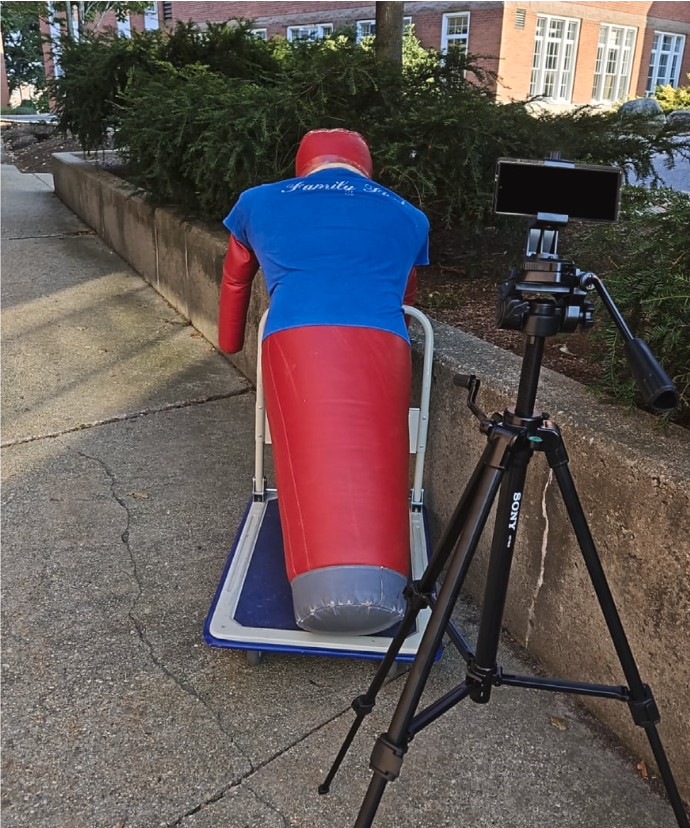
\includegraphics[width=0.5\textwidth]{img/dummy.png}
    \caption{Experimental setup using a grappling dummy to simulate fall events for the SAFE dataset.}
    \label{fig:grappling_dummy}
\end{figure}

\subsubsection{Evaluation Methodologies}
Evaluation metrics are a key part of ensuring reproducibility and facilitating direct comparisons across studies. For the purpose of this thesis, the identical metrics will be utilized as defined in the original study of the paper ``SAFE: Sound Analysis for Fall Event detection using machine learning. These metrics will be outlined in this section, including brief descriptions and their mathematical formulas.

To understand these metrics, the components of the confusion matrix must first be defined.
\begin{itemize}
    \item \textbf{True Positive (TP):} A fall occurs, and the model correctly detects it.
    \item \textbf{True Negative (TN):} No fall occurs, and the model correctly predicts no fall.
    \item \textbf{False Positive (FP):} No fall occurs, but the model incorrectly detects a fall (False Alarm).
    \item \textbf{False Negative (FN):} A fall occurs, but the model fails to detect it (Missed Detection).
\end{itemize}



The most popular metric in binary supervised machine learning is \textbf{Accuracy}. It is simply the number of correctly predicted records divided by the total number of records, and it is defined as:

\begin{equation}
\text{Accuracy} = \frac{TP + TN}{TP + TN + FP + FN}
\end{equation}

Although accuracy is a useful metric, it can be misleading for imbalanced data, which is common in fall datasets. Moreover, it does not provide sufficient granularity to fully understand the outcome.

\textbf{Recall} (also known as Sensitivity) measures the proportion of true positives identified among all actual positives. It is calculated as:

\begin{equation}
\text{Recall} = \frac{TP}{TP + FN}
\end{equation}

This is a critical metric in event detection, as it indicates the percentage of actual falls the system detects among all fall events.

\textbf{Precision} measures the proportion of true positives among all instances predicted as positive. It is defined as:

\begin{equation}
\text{Precision} = \frac{TP}{TP + FP}
\end{equation}

It is important for the model to have high precision to minimize false positives, which creates a burden for nurses and assistants helping the patients.

\textbf{F1-score} is the harmonic mean of Precision and Recall. It provides a single metric that balances both concerns and is given by:

\begin{equation}
\text{F1-score} = 2 \times \frac{\text{Precision} \times \text{Recall}}{\text{Precision} + \text{Recall}}
\end{equation}


\subsection{Summary and Research Gap}
\label{summa}
This literature review provided an overview of the fall detection domain, with a focus on methods. Firstly, the clinical context outlined that this topic is paramount, as many people suffer falls each year. The overview of different approaches showed that fall detection is well investigated, and wearable-based strategies are the most ubiquitous. This strategy was compared with both acoustic sensing and vision-based sensing. Though it is a robust technique, it is dependent on user compliance, making it a burden for people who face challenges maintaining technological equipment. The vision-based approach showed great potential but has a major privacy issue, especially in rooms like bedrooms and bathrooms, where falls are most common. Consequently, the audio-based approach mitigates all these issues, making it a very promising strategy that is user-friendly and preserves privacy. The signal feature space requires complex processing, and the data can be better used after feature extraction, a necessary step for providing time-domain, frequency-domain, and time–frequency representations such as MFCCs and Mel spectrograms. The current state of this domain has shifted from classical machine learning to deep learning, making the strategy more computationally intensive. Though the results are exemplary in lab environments, they are not robust, they struggle with generalization, and they underperform in real-world scenarios. These gaps motivate the focus of this thesis on lightweight audio-based fall detection models, robust preprocessing pipelines, and evaluation on publicly available datasets. Unfortunately, data scarcity is a major limitation in this domain, and most researchers use their own custom datasets. There are a few datasets available, such as the SAFE dataset, which contains 950 audio samples. 

/subsection{additional remarks to be added}
\subsubsection{Alignment Strategy for Heterogeneous Datasets}
To facilitate a direct, scientific comparison between the SAFE dataset and the augmented hard negatives derived from the ESC-50 corpus, a standardized alignment strategy was implemented. While the SAFE dataset consists of 3-second clips with the fall event centered [cite: 567], the ESC-50 samples are 5 seconds in length with variable event onsets[cite: 588]. 

To mitigate the risk of temporal bias, all 5-second distractor clips were processed using an impact-centered cropping algorithm. The center of the event was identified by calculating the Short-Time Energy (STE) across the signal to locate the point of maximum impulsive power $t_{peak}$[cite: 358]:

\begin{equation}
E_n = \sum_{m} [x[m] \cdot w[n-m]]^2
\end{equation}

A 3-second window was then extracted, defined by the interval $[t_{peak} - 1.5s, t_{peak} + 1.5s]$. This ensures that the impulsive characteristics of both falls and hard negatives are positioned identically within the input buffer. This alignment is critical for the feature extraction phase, particularly for calculating time-frequency representations like Mel-spectrograms [cite: 393, 408], ensuring that the model differentiates classes based on their spectral decay and frequency distribution rather than temporal positioning[cite: 281].

% \subsection{Existing Methods and Algorithms}
% \subsection{Environments and Libraries}
% \subsection{Challenges in Audio-Based Fall Detection}

% \section{Methods}
% \subsection{Proposed Novel Solutions}
% \subsection{Thesis Objectives}
% \subsection{System Architecture}
% \subsection{Implementation Details}

% \section{Results}
% \subsection{Data Sets Description}
% \subsection{Experimental Results}
% \subsection{Comparison with Related Techniques}
% \subsection{Discussion of Key Findings}

% \section{Summary}
% \subsection{Key Findings}
% \subsection{Limitations of the Solution}
% \subsection{Future Works}

% --- 6. BIBLIOGRAPHY ---
\printbibliography[heading=bibintoc, title={Bibliography}]

% --- 7. LISTS ---
% Note: Changed 'chapter' to 'section' for TOC levels
\section*{List of Symbols and Abbreviations}
\addcontentsline{toc}{section}{List of Symbols and Abbreviations}
\begin{tabbing}
    \hspace{4cm} \= \kill
    \textbf{ML} \> Machine Learning \\
    \textbf{ANN} \> Artificial Neural Network
\end{tabbing}

\listoffigures
\addcontentsline{toc}{section}{List of Figures}

\listoftables
\addcontentsline{toc}{section}{List of Tables}

\section*{List of Appendices}
\addcontentsline{toc}{section}{List of Appendices}
\noindent
Appendix A: Python Source Code Structure \\
Appendix B: Additional Experiment Results

% --- 8. APPENDICES ---
\appendix
% In 'article' class, \appendix changes \section numbering to A, B, C...

\section{Python Source Code Structure}
[Content]

\section{Additional Experiment Results}
[Content]

\end{document}